\documentclass[nomenclature, norefpage, oneside, glossary, hypertext,multiauthor]{hsmw-class}

% Optionen:
% 150 -> Jubiläums Logo 
% nomenclature -> Abkürzungsverzeichnis
% norefpage -> Abkürzungsverzeichnis ohne Seitenverweis
% oneside -> kein zweiseitiges Druckbild
% glossary -> Glossar für Begriffe
% hypertext -> Links im PDF
% multiauthor -> mehrere Autoren in \Autorenteam{}
% english -> English Layout
% index -> fügt einen Index ein

% für Umlaute (UTF8 Zeichensatz)
\usepackage[utf8]{inputenc}  

% für Anführungszeichen mit \enquote{...}
\usepackage[autostyle=true,german=quotes]{csquotes}

% für das Literaturverzeichnis
\usepackage[
hyperref=true, % Links zu Referenzen
style=authoryear, % Autor/Jahr Zitierweise
natbib, % Formatierengine
giveninits=true, % Initialien für Vornamen
dashed=false, % wenn true, werden wiederholte Erstautorennamen
              % mit - ersetzt 
maxbibnames=10, % ab wann soll et al. gedruckt werden
terseinits=true, % Initialien ohne Punkt und Leerzeichen
uniquename=init, %
]{biblatex} 



% Lädt Bibliograpie aus Datei literatur.bib
\addbibresource{hsmw-literatur.bib}

% Ersetzt u.a. mit et al.
\DefineBibliographyStrings{ngerman}{andothers={{et\,al\adddot}}} 

% Ignoriert Sonderzeichen im Abstract in .bib-Datei
\DeclareSourcemap{
  \maps[datatype=bibtex]{
    \map{
       \step[fieldset=abstract, null]
    }
 }
}

% Erstellt den Filter "original" für Literaturverzeichnis
\defbibfilter{original}{
  type=article or
  type=inproceedings or
  type=inbook or
  type=book
}


%%%%%%%%%%

\Art{Handreichung} % Protokoll / Bachelorarbeit / Masterarbeit / ...

\Anrede{Organisationseinheit} % Herr/Frau

% Einzelautor - aktiv ohne multiauthor Option
\Vorname{Frida}
\Nachname{Engel}

% Autorenteam - aktiv bei multiauthor Option
\Autorenteam{Fachgruppe Biotechnologie und Chemie}


\Thema{Vorlage und Informationen für das Verfassen von Protokollen und Abschlussarbeiten}
\Unterthema{Für alle \LaTeX{}-Freunde}

% Ihr Studiengang:
\Studiengang{Bachelor Biotechnologie\\Master Genomische Biotechnologie}

% Ihre Seminargruppe
\Seminargruppe{}

\Fakultaet{} % Voreinstellung: CB

\Erstpruefer{} % Prof. der Hochschule Mittweida
\Zweitpruefer{} % Externer Betreuer

\WeitererBetreuer{} % 

\Datum{} % für Selbstständigkeitserklärung

\Tag{}
\Monat{}
\Jahr{} % für Titelseiten und bibliographische Angaben

% Nach Bedarf für die bibliographische Angaben füllen
\Anlagen{} % zB CDROM
\Copyright{}
\Textsatz{\LaTeX{}}
\Druck{}
\Verlag{}
\ISBN{}

% Englischer Titel - IMMER ANGEBEN
\TitelZwei{Template for and Information about Writing Protocols and Final Theses}



\begin{document} %%%%%%%%%%%%%%%%%%%%%%%%%%%%%%%%%%%%%%%%%%%%%%

% Datei mit dem Glossar - aktiv mit Option glossary
\input{hsmw-glossar.txt}

% Datei mit dem Abkürzungsverzeichnis - aktiv mit Option nomenclature
\input{hsmw-abk.txt}

\begin{Kurzbeschreibung}
Die Kurzbeschreibung, gelegentlich auch Referat genannt, im englischen \textit{Abstract}, enthält eine Zusammenfassung der Arbeit in wenigen Sätzen. Die Kurzbeschreibung ersetzt nicht die Zusammenfassung der Arbeit.
\end{Kurzbeschreibung}

% Ein Vorwort ist bei Protokollen und Abschlussarbeiten unüblich
%\begin{Vorwort}
%Text Vorwort
%\end{Vorwort}

% Eine Danksagung ist bei Abschlussarbeiten üblich
\begin{Danksagung}
Eine Danksagung ist bei Abschlussarbeiten üblich. Sie gehört aber nicht in Protokolle. Denken Sie daran, dass die Danksagung Teil der öffentlich zugänglichen Abschlussarbeit ist. Sie sollte ernsthaft formuliert sein und sie sollten nicht ihrem Goldhamster Danken.

Ich möchte an dieser Stelle Professor Klaus Dohmen für die gute Vorlage danken, die Professor Wünschiers zu dieser \enquote{bio-spezifischen} Vorlage erweitert hat.
\end{Danksagung}


\Hauptteil % Diese Anweisung nicht löschen!

\chapter{Über diese \LaTeX{}-Vorlage}
Nachfolgend finden Sie eingige wichtige Informationen zu dieser Vorlage. Eine gute Online-Einführung finden sie unter \url{de.wikibooks.org/wiki/LaTeX-Kompendium}. Ein superkurze Einführung ist auch in meinem Buch enthalten \citep{Wuenschiers2016kap12}.
Scheuen Sie sich nicht, mich (Röbbe Wünschiers) auf Fehler und Verbesserungsvorschläge hinzuweisen.

In einer älteren Version konnte es zu dem LaTeX Error »File 'scrpage2.sty' not found.« kommen. Infolgedessen wurde keine PDF-Datei erzeugt. Das \textit{scrpage2}-Paket ist für die Beschriftung der Seitenköpfe zuständig und veraltet. Ich habe es durch das Paket \textit{scrlayer-scrpage} in der Datei \textit{hsmw-class.cls} ersetzt.

\section{Notwendige Dateien}
Diese Vorlage besteht aus mehreren Dateien, die alle im selben Verzeichnis liegen müssen. Diese sind ...

\begin{tabular}{lp{.6\textwidth}}
\textit{hsmw-vorlage.tex} & Die Hauptdatei, die Ihren Text enthält \\
\textit{hsmw-class.cls} & Die Style-Datei, welche die Formatierung bestimmt.\\
\textit{hsmw-counter.sty} & Enthält wichtige Zähler für Kapitel usw.\\
\textit{biblatex.cfg} & Konfiguration für Literaturverzeichnis\\
\textit{hsmw-glossar.txt} & Datei mit den Begriffen und Definitionen für das Glossar.\\
\textit{hsmw-abk.txt} & Datei mit den Begriffen und Definitionen für das Abkürzungsverzeichnis.\\
\textit{hsmw-literatur.sty} & Datei für das Literaturverzeichnis.\\
\textit{hsmw-logo.pdf} & Das Hochschulelogo\\
\textit{hsmw-logo-150.pdf} & Das Jubiläums-Hochschullogo\\
\textit{fig-latex.png} & eine Abbildung\\
\end{tabular}

\section{Formatierungsoptionen}
In der ersten Zeile der Vorlage \textit{hsmw-vorlage.tex} wird die Dokumentenklasse \textit{hsmw-class}  mit \verb+\documentclass[OPTIONEN]{hsmw-class}+ aufgerufen. Dabei stehen Ihnen zahlreichen OPTIONEN zur Verfügung:

\begin{tabular}{lp{.6\textwidth}}
\texttt{multiauthor} & Stellt den Befehl \verb+\Autorenteam{}+ für mehrere Autoren (bei Protokollen) zu Verfügung \\
\texttt{oneside} & kein doppelseitiges Druckbild \\
\texttt{nomenclature} & Erstellung eines Abkürzungsverzeichnis \\
\texttt{norefpage} & Abkürzungsverzeichnis ohne Seitenverweis \\
\texttt{hypertext} & Erzeugt Links im PDF \\
\texttt{glossary} & Erstellung eines Glossars \\
\texttt{english} & Englische Kapitelüberschriften \\
\texttt{index} & fügt einen Index ein \\
\texttt{150} & Verwendung des Jubiläumslogos \\
\end{tabular}


\section{Abkürzungsverzeichnis}
Das Abkürzungsverzeichnis ist sehr wichtig und wird mit der Option \texttt{nomenclature} aktiviert. Die Begriffe sind in die Datei \textit{hsmw-abk.txt} einzutragen.


\section{Einfügen von URLs}
Verwenden Sie für Webseiten den Befehl \verb+\url{}+, dann sehen Links (\url{http://datenmassen.de}) gut aus.

\section{Abbildungen \& Tabellen} \label{sec-abb}
Abbildungen und Tabellen müssen immer im Text referenziert werden. Dazu erstellen Sie mit \verb+\label{}+ eine Marke, auf die Sie woanders im Text mit \verb+\ref{}+ verweisen können.

Die Abb. \ref{fig:latex} zeigt das \LaTeX{}-Dokument, mit dem wir im Modul \enquote{Wissenschaftliches Schreiben} begonnen haben. Abbildungen können Sie als PDF- oder PNG-Datei hinterlegen.

\begin{figure}[h]
    \centering
    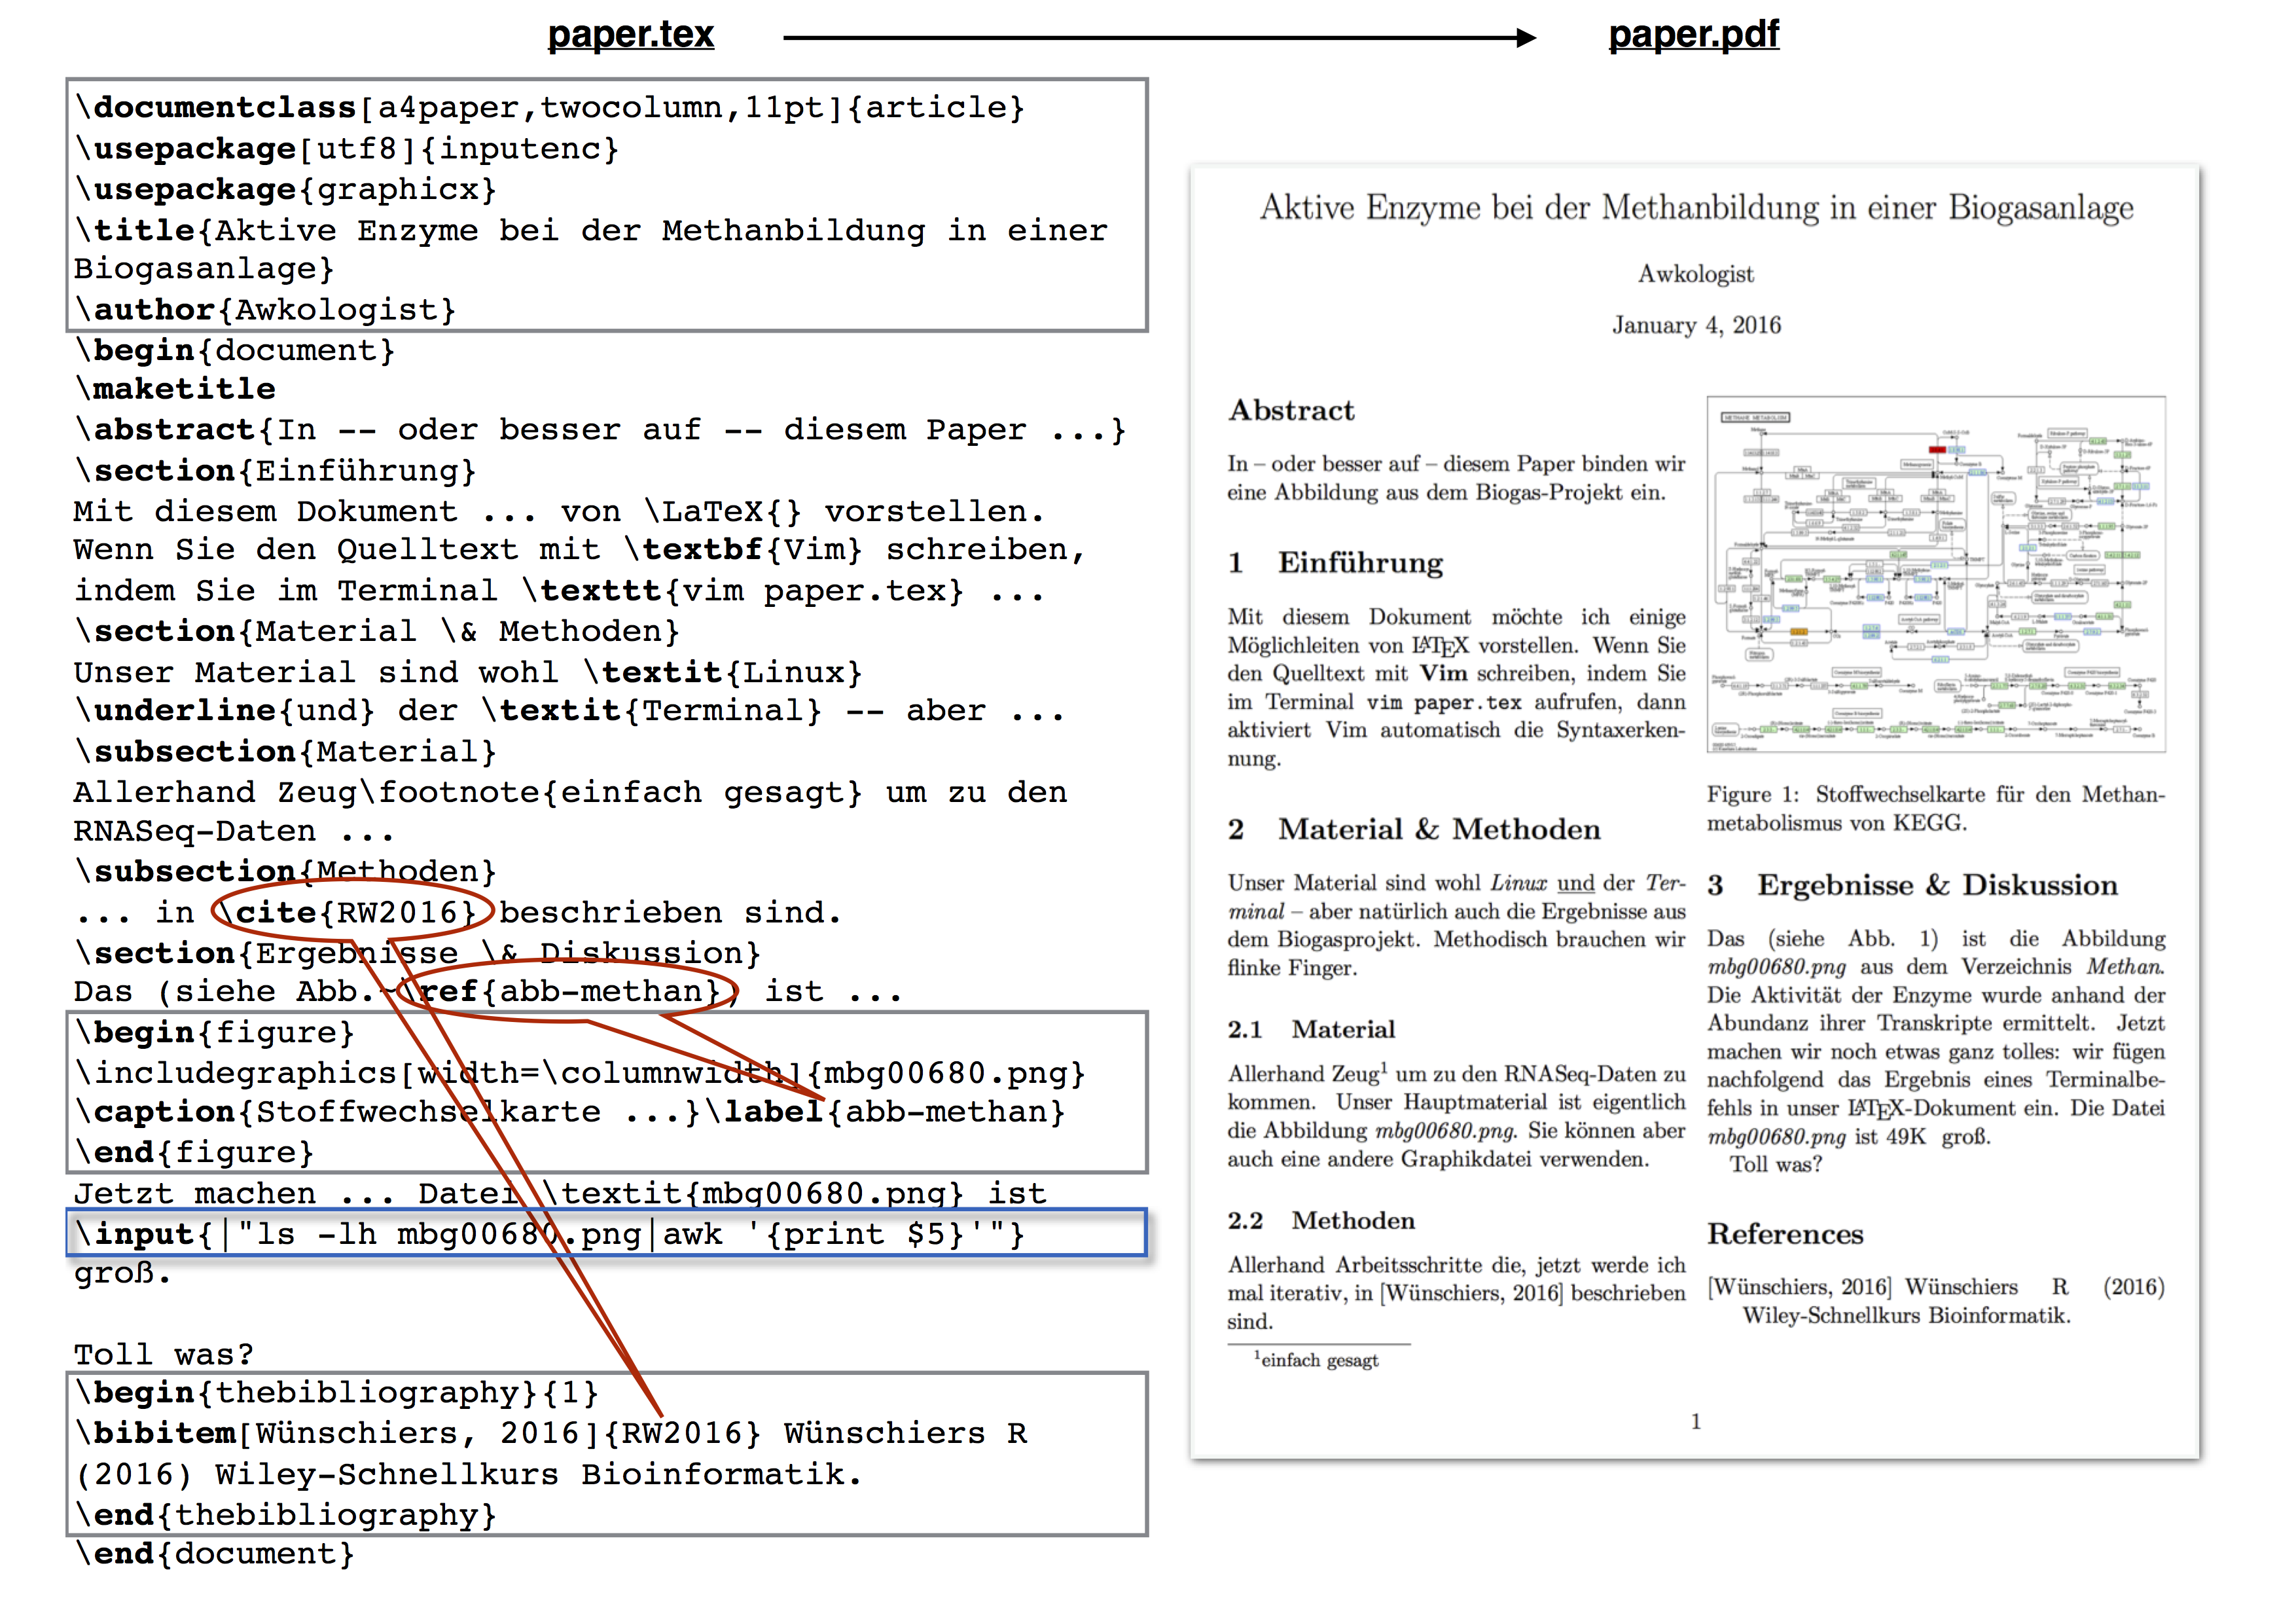
\includegraphics[width=.7\columnwidth]{fig-latex.png}
    \caption{Von \LaTeX{} zum PDF. Aus \citep{Wuenschiers2016}}.
    \label{fig:latex}
\end{figure}

Für Abbildungen verwenden Sie die Umgebung \texttt{figure}, wie im Beispiel in der Datei \textit{hsmw-vorlage.tex} angewendet. 

Tabellen können beliebig komplex werden. Ein einfaches Beispiel ist in Tab. \ref{tab:mendel} zu sehen.

\begin{table}
\centering
\begin{tabular}{cccccc}
\hline
\multicolumn{3}{c}{1. Versuch} &  & \multicolumn{2}{c}{2. Versuch}\\
\multicolumn{3}{c}{Gestalt der Samen} & & \multicolumn{2}{c}{Färbung }\\
& & & & \multicolumn{2}{c}{des Albumens}\\
Pflanze & rund & kantig &   &  gelb &  grün  \\
\cline{1-3} \cline{5-6} \\
1 & 45 & 12 &   &  25 &  11  \\
2 & 27 & 8 &   &  37 &  7  \\
... & ... & ... &   &  ... &  ...  \\
10 & 25 & 7 &   &  44 &  18  \\
\hline
\end{tabular}
\caption{Eine Tabelle mit Ergebnissen aus den Versuchen von Gregor Mendel \citep{Mendel1866}.}
\label{tab:mendel}
\end{table}

 
\section{Bibliographie}
Literatur zitieren Sie entweder in Klammern mit dem Befehl \verb+\citep{}+\citep{Huang1976,Wuenschiers2004,Stark2014} oder im Text mit \verb+\citet{}+, wie folgendes fiktives Beispiel zeigt: Ausserdem konnten \citet{Kanai2017} zeigen, dass \citep{ford} falsch lag \citep{Jing2016}.

Biblatex-formatierte Referenzen können zum Beispiel mit JabRef (\url{http://www.jabref.org}) erstellt werden und müssen in die Datei \textit{hsmw-literatur.bib} eingetragen werden.
 

\section{Glossar}
Wenn Sie ein Glossar verwenden möchten, dann müssen Sie die Option \texttt{glossary} verwenden und die Begriffe in die Datei \textit{hsmw-glossar.txt} schreiben. In dieser Datei finden Sie ein Beispiel für \gls{befruchtungen}. 


\section{Index}
Ein Index wird eigentlich nur in Büchern verwendet und sei hier nur der Vollständigkeit halber erwähnt. Mit der Option\index{Option} \texttt{index} steht Ihnen der Befehl \verb+\index{}+ zur Verfügung.


\chapter{Allgemeine Informationen}
Ein Kapitel (\verb+\chapter{}+) beginnt immer auf einer neuen Seite.

Allgemeine Informationen werde ich später einmal diesem Dokument hinzufügen. Aktuell finden Sie Hinweise unter \url{http://www.cb.hs-mittweida.de/webs/biotechnologie/abschlussarbeiten.html#c25741}.



\Anhang


% Befehl für ein Gesamtliteraturverzeichnis
%\printbibliography

% Befehle für getrennte Verzeichnisse; der Filter original ist im Dokumentenkopf definiert (article, inproceedings, book)
\printbibliography[filter=original, title={Originalarbeiten}]
\printbibliography[type=online, title={Webseiten}]


\end{document}
